
\chapter{Consumers, producers, and the efficiency of markets}

\keyword{welfare economics}: the study of how the allocation of resources affect economic well-being.


\section{Consumer surplus}

\subsection{Willingness to pay}

Each buyer's maximum price is called his \keyword{willingness to pay}, and it measures how much that buyer values the good.

\keyword{Consumer surplus} is the amount a buyer is willing to pay for a good minus the amount the buyer actually pays for it.
Consumer surplus measures the benefit to buyers of participating in a market.

\subsection{Using the demand curve to measure consumer surplus}

The demand curve is shown in Figure \ref{fig:the-demand-curve}:

\begin{figure}[!ht]
  \centering
  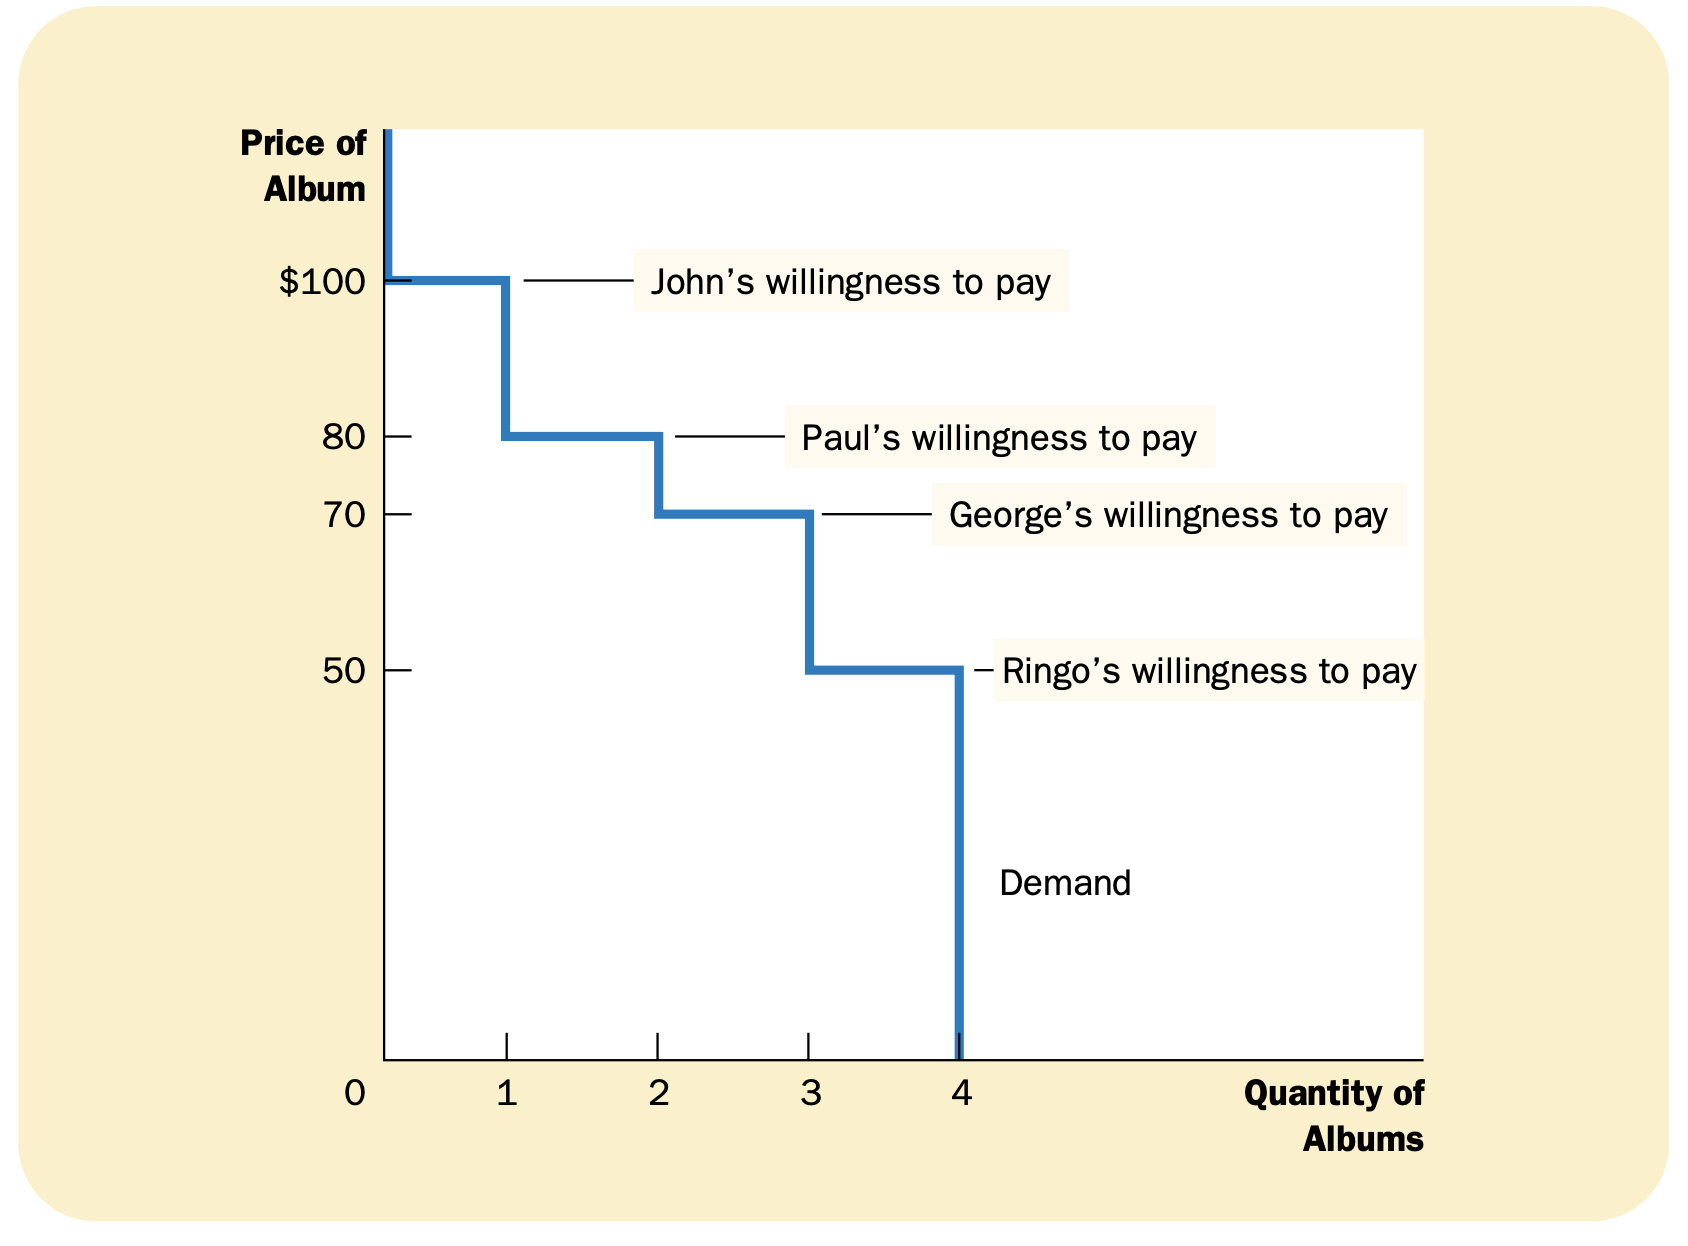
\includegraphics[width=\textwidth]{pics/willingness-to-pay}
  \caption{The demand curve}
  \label{fig:the-demand-curve}
\end{figure}

At any quantity, the price given by the demand curve shows the willingness to pay of the \keyword{marginal buyer},
the buyer who would leave the market first if the price were any higher.


Because the demand curve reflects buyers’ willingness to pay, we can also use it to measure consumer surplus.
Figure \ref{fig:consumer-surplus} uses the demand curve to compute consumer surplus.
Figure \ref{fig:consumer-surplus} shows that:
\keyword{The area below the demand curve and above the price measures the consumer surplus in a market.}
\begin{figure}[!ht]
  \centering
  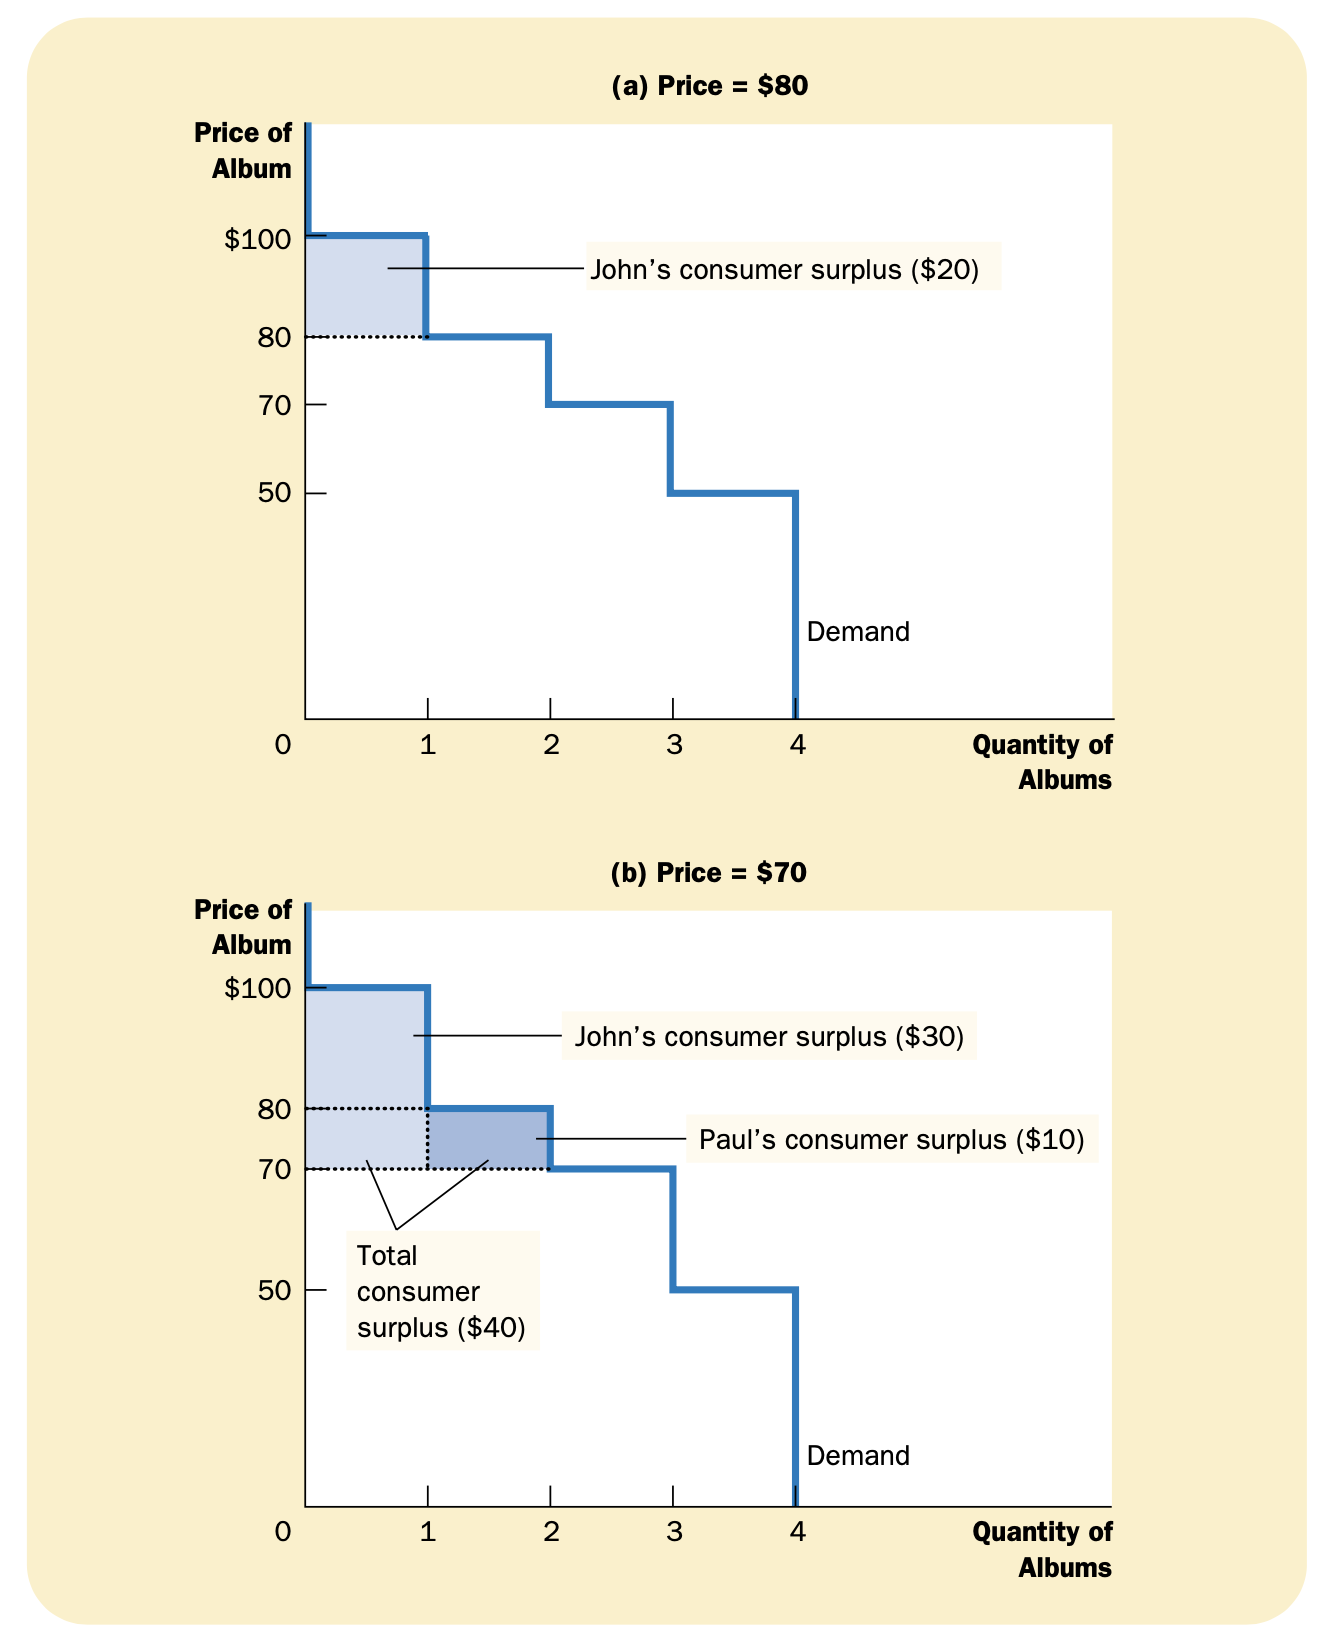
\includegraphics[width=\textwidth]{pics/consumer-surplus}
  \caption[Consumer surplus]{Measuring consumer surplus with the demand curve}
  \label{fig:consumer-surplus}
\end{figure}

\subsection{How a lower price raise consumer surplus}

\begin{figure}[!ht]
  \centering
  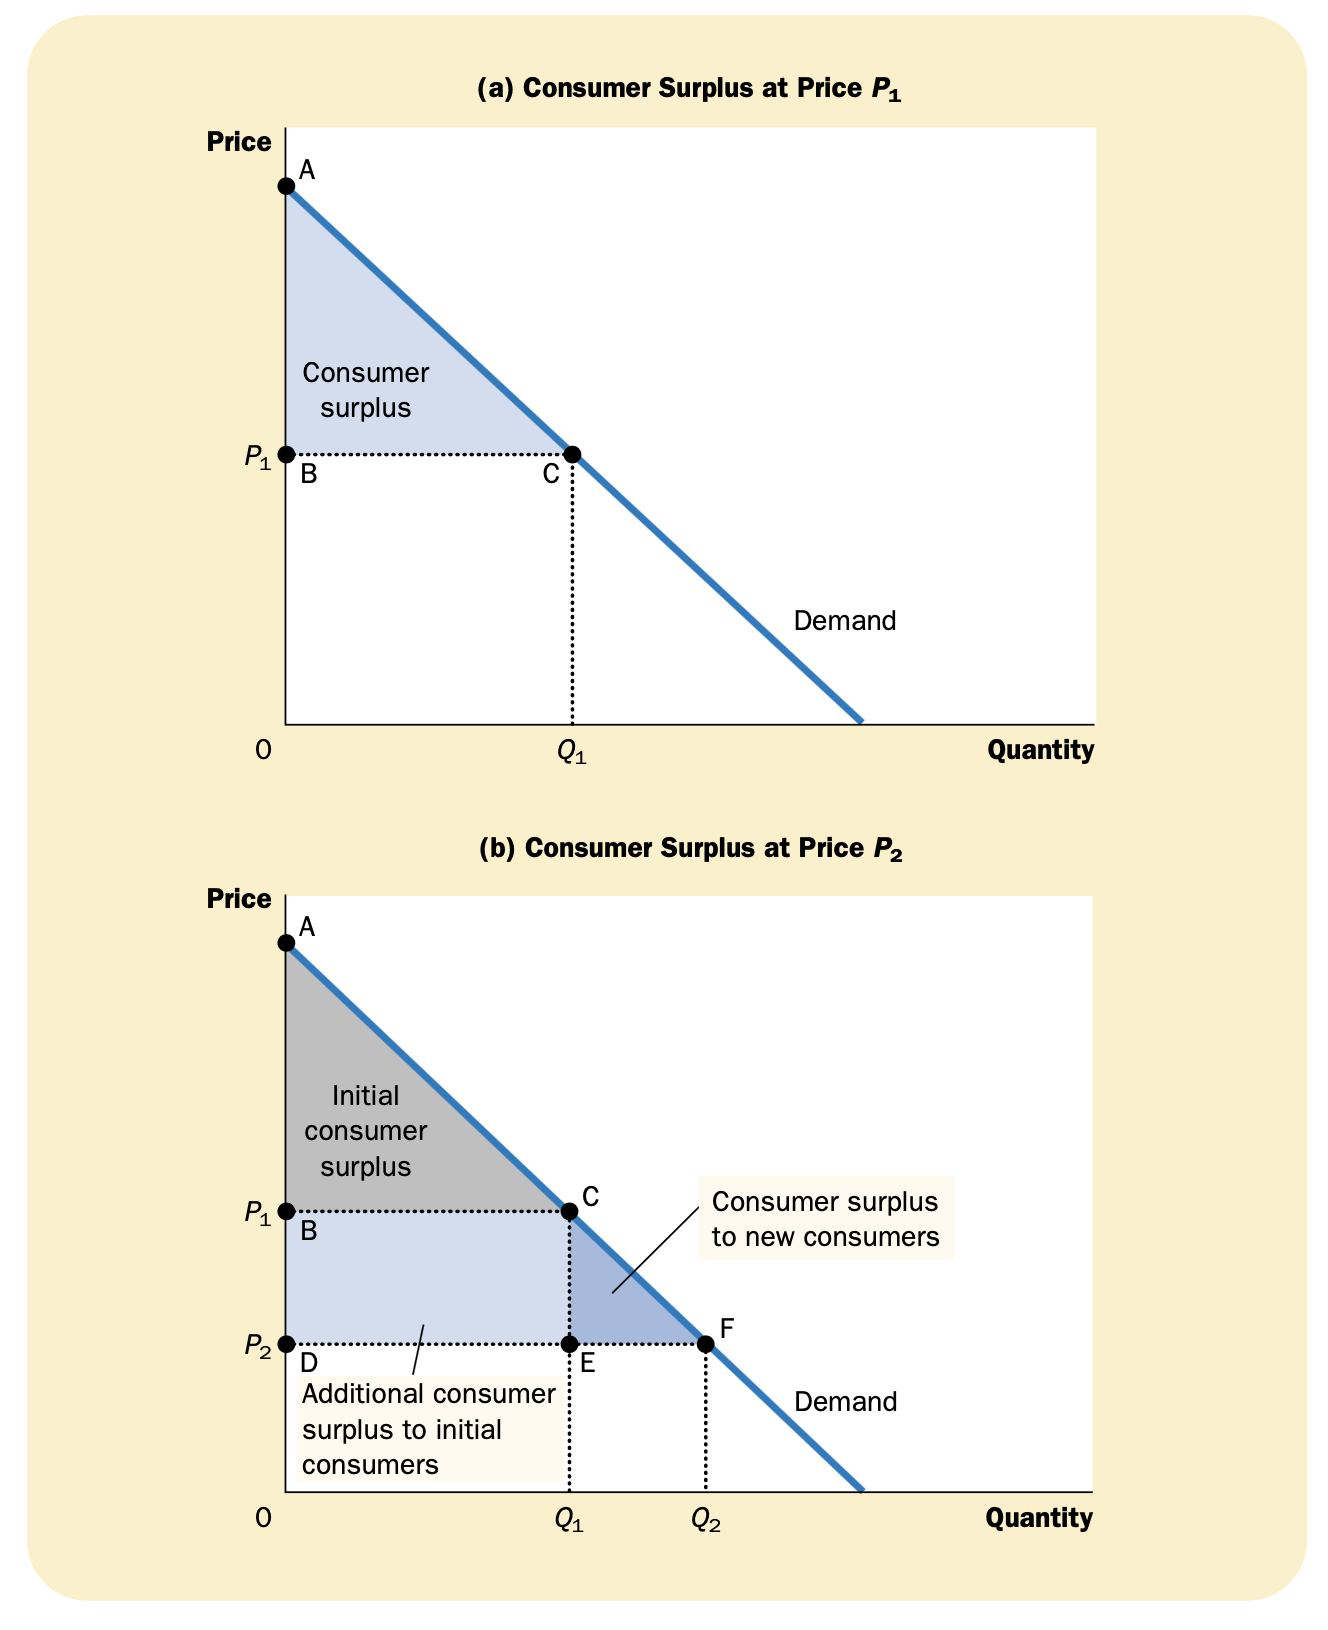
\includegraphics[width=\textwidth]{pics/consumer-surplus2}
  \caption{How the price affects consumer surplus}
  \label{fig:consumer-surplus2}
\end{figure}


\subsection{What does consumer surplus measure?}

In most markets consumer surplus does reflect economic well-being.
Economists normally presume that buyers are \keyword{rational} when they make decisions and that their preferences should be respected.
In this case, consumers are the best judges of how much benefit they receive from the goods they buy.



\section{Producer surplus}

\subsection{Cost and the willingness to sell}

\keyword{Producer surplus} is the amount a seller is paid minus the cost of production.
Producer surplus measures the benefit to sellers of participating in a market.


\subsection{Using the supply curve to measure producer surplus}

\begin{figure}[!ht]
  \centering
  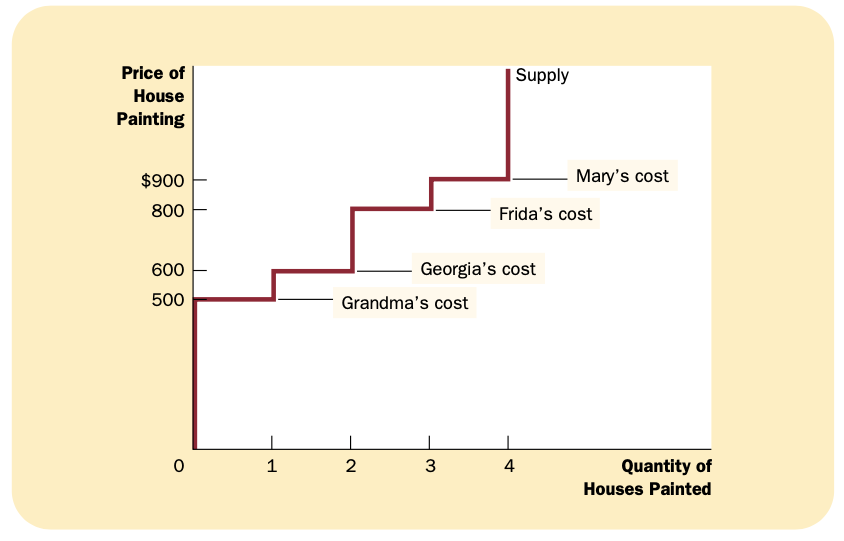
\includegraphics[width=\textwidth]{pics/the-supply-curve}
  \caption{The supply curve}
  \label{fig:the-supply-curve}
\end{figure}

Figure \ref{fig:the-supply-curve} shows the supply curve.
At any quantity, the price given by the supply curve shows the cost of the \keyword{marginal seller},
the seller who would leave the market first if the price were any lower.


Because the supply curve reflects sellers’ costs, we can use it to measure producer surplus.
Figure \ref{fig:the-producer-surplus} uses the supply curve to compute producer surplus in our example.
Figure \ref{fig:the-producer-surplus} shows that:
\keyword{The area below the price and above the supply curve measures the producer surplus in a market.} 
\begin{figure}[!ht]
  \centering
  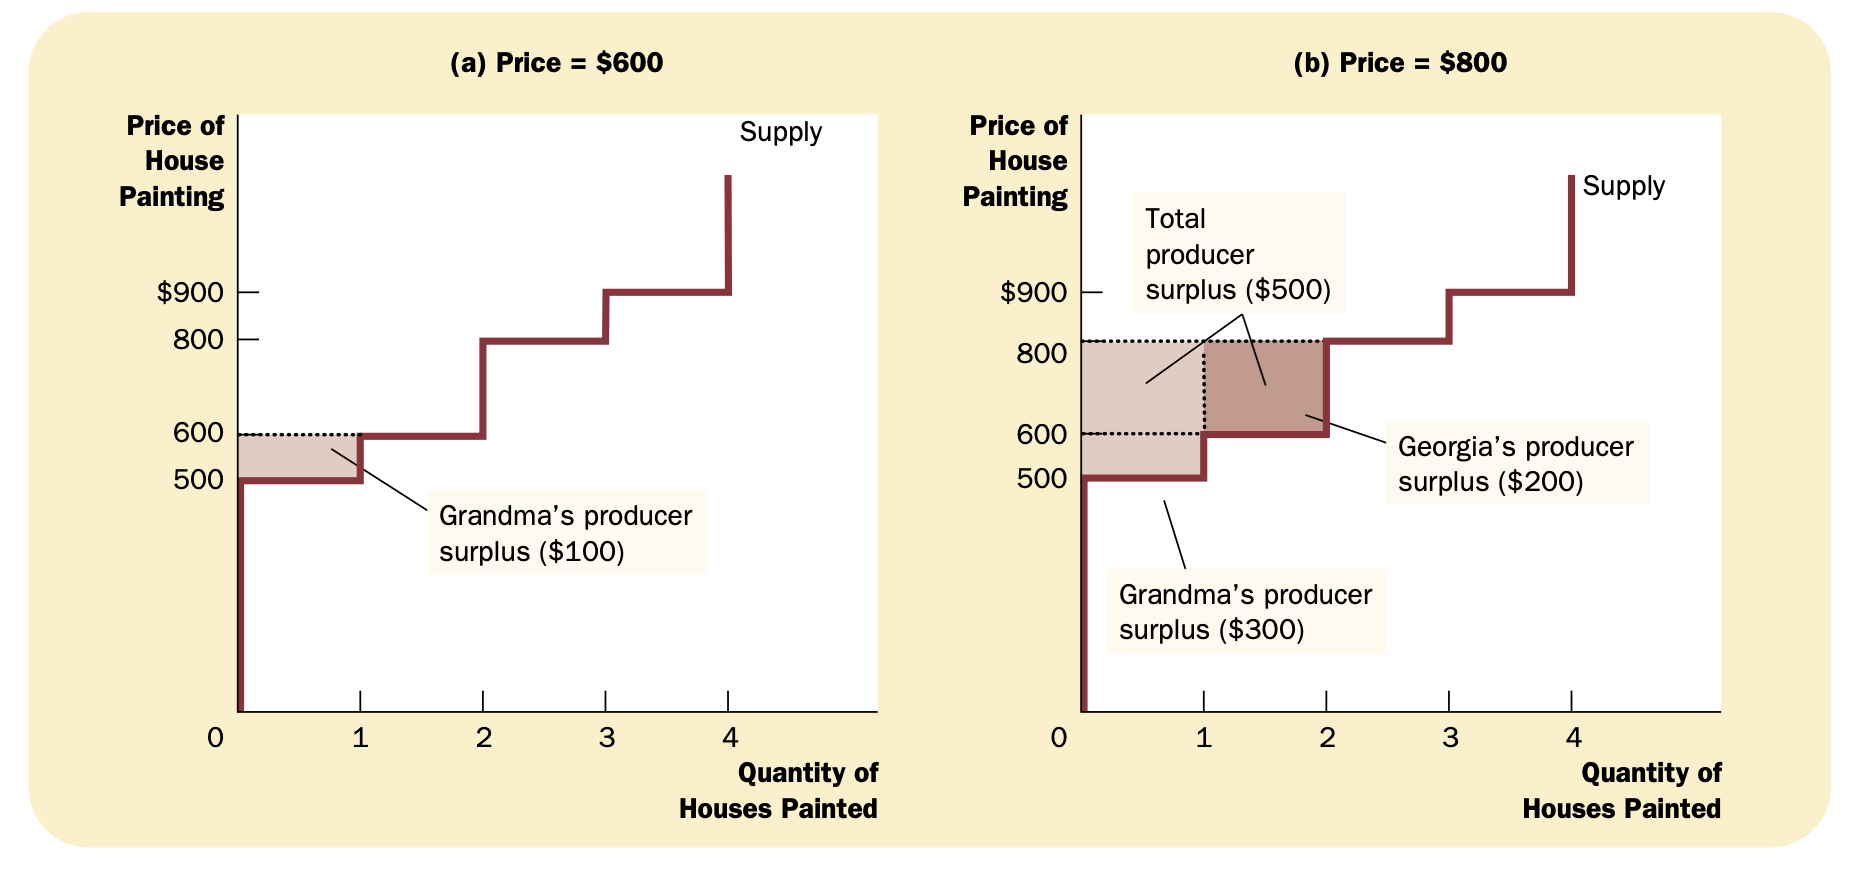
\includegraphics[width=\textwidth]{pics/producer-surplus}
  \caption{The producer surplus}
  \label{fig:the-producer-surplus}
\end{figure}


\subsection{How a higher price raises producer surplus}

\begin{figure}[!ht]
  \centering
  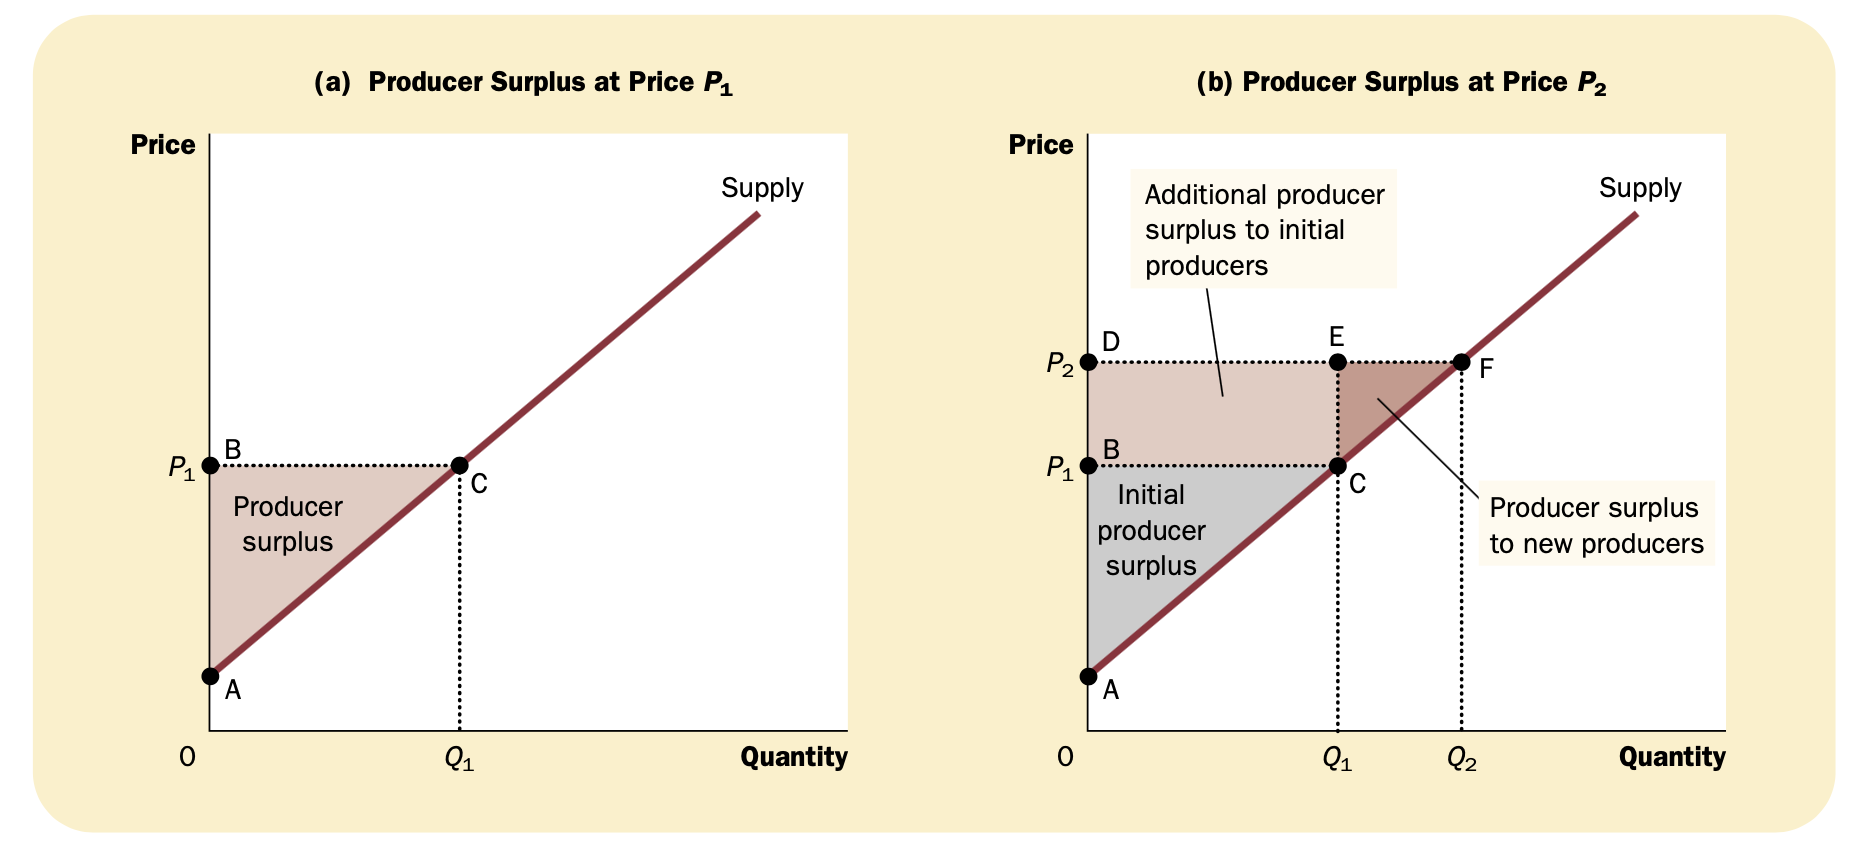
\includegraphics[width=\textwidth]{pics/producer-surplus2}
  \caption{HOW a higher price raises producer surplus}
  \label{fig:the-producer-surplus2}
\end{figure}


\section{Market efficiency}

\begin{equation}
  \text{Consumer surplus} = \text{Value to buyers} - \text{Amount paid by buyers}.
\end{equation}
\begin{equation}
  \text{Producer surplus} = \text{Amount received by sellers} - \text{Cost to sellers}.
\end{equation}


When we add consumer and producer surplus together, we obtain
\begin{equation}
  \text{Total surplus} = \text{Value to buyers} - \text{Amount paied by buyers}
  + \text{Amount received by sellers} - \text{Cost to sellers}.
\end{equation}

The amount paid by buyers equals the amount received by sellers, so the middle two terms in this expression cancel each other.
As a result, we can write total surplus as
\begin{equation}
  \text{Total surplus} = \text{Value to buyers} - \text{Cost to sellers}.
\end{equation}

If an allocation of resources maximizes total surplus, we say that the allocation exhibits \keyword{efficiency}.


\subsection{Evaluating the market equilibrium}

Figure \ref{fig:market-equilibrium} shows consumer and producer surplus when a market reaches the equilibirm of supply and demand.

\begin{figure}[!ht]
  \centering
  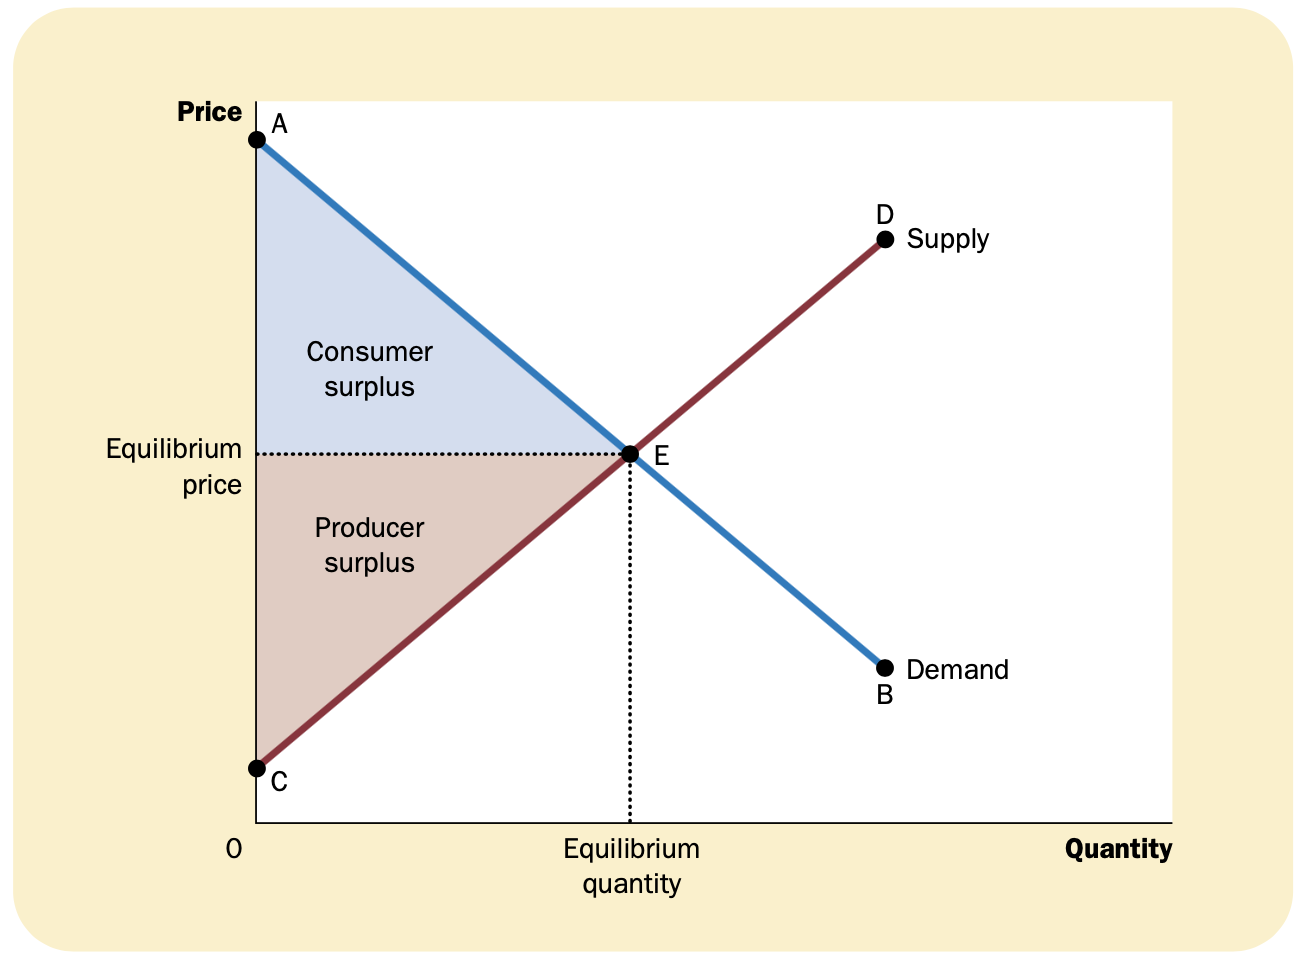
\includegraphics[width=\textwidth]{pics/market-equilibrium}
  \caption[Surplus in market]{Consumer and producer surplus in the market}
  \label{fig:market-equilibrium}
\end{figure}

Is this equilibrium allocation of resources efficient?
Does it maximize total surplus?

To answer these questions, keep in mind that
when a market is in equilibrium, the price determines which buyers and sellers participate in the market.
Those buyers who value the good more than the price (represented by the segment AE on the demand curve) choose to buy the good;
those buyers who value it less than the price (represented by the segment EB) do not.
Similarly, those sellers whose costs are less than the price (represented by the segment CE on the supply curve) choose to produce and sell the good;
those sellers whose costs are greater than the price (represented by the segment ED) do not.



These observations lead to two insights about market outcomes:
\begin{enumerate}
\item Free markets allocate the supply of goods to the buyers who value them most highly, as measured by their willingness to pay.
\item Free markets allocate the demand for goods to the sellers who can produce them at least cost.
\item Free markets produce the quantity of goods that maximizes the sum of consumer and producer surplus.
\end{enumerate}


To see why this is true, consider Figrue \ref{fig:market-equilibrium2}.

\begin{figure}[!ht]
  \centering
  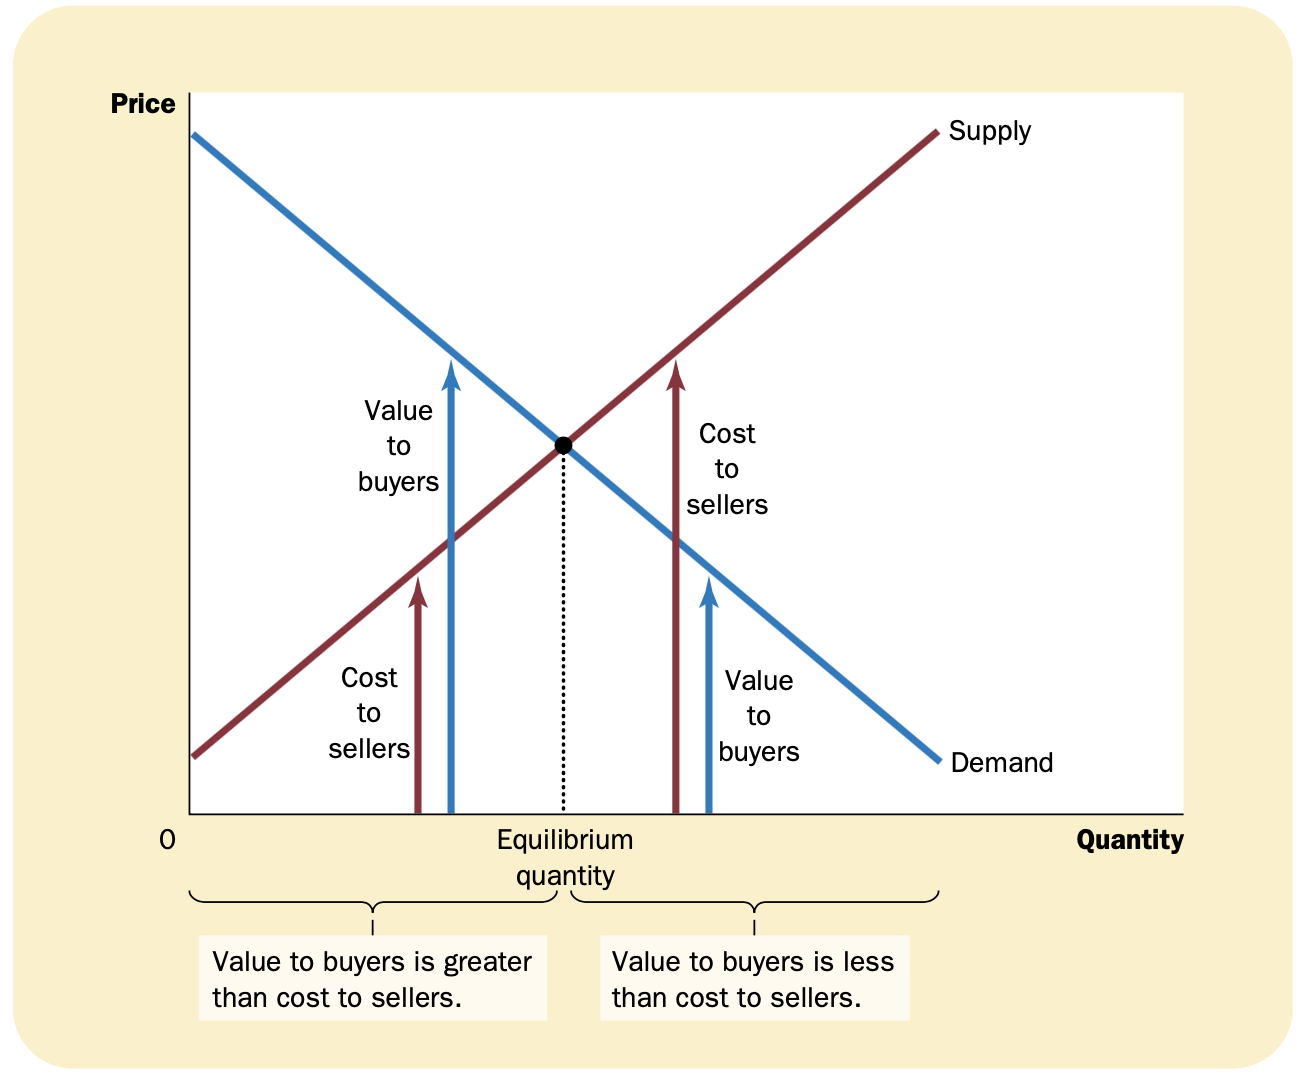
\includegraphics[width=\textwidth]{pics/market-equilibrium2}
  \caption[Efficiency]{The efficiency of the equilibrium quantity}
  \label{fig:market-equilibirum2}
\end{figure}